\documentclass{unswmaths}
\usepackage{mathtools}
\usepackage{unswshortcuts}


\author{Adam J. Gray}
\studentno{3329798}
\subject{Fractional Differential Equations}
\title{Honours Thesis}
\supervisor{Dr Chris Tisdell}


\begin{document}

\unswtitle

\setlength\parindent{0pt}
\setlength{\parskip}{5mm plus4mm minus3mm}

%\tableofcontents

\section*{Introduction}
%\addcontentsline{toc}{section}{Introduction}
\subsection*{Historical Overview and Motivation}
\subsubsection*{Prehistory: Liebniz to Fourier}
Although one can argue that fractional calculus is a field which is essentially as old as
``conventional'' calculus iteslef we will regard all development in the field up until the
work of Abel as prehistory. This is because the first applications of the field did not appear
until Abel and even simple definitions were not properly developed.

\subsubsection*{L'Hopital \& Liebniz}
Leibniz, in reply to L'Hopital's question about the operator $ \frac{d^\frac{1}{2}}{dx^\frac{1}{2}} $, 
wrote, ``It will lead to a paradox, from which one day useful consequences will be drawn.''
\subsubsection*{Leibniz, Wallis \& Bernoulli}
Leibniz, in letters addressed to John Wallis and Daniel Bernoulli in 1697, proposed a 
formulation for the fractional derivitive of an exponential function.
He proposed that 
$$
    \frac{d^r}{dx^r} e^{mx} = m^r e^{mx}.
$$
Keeping in mind that this is was the late 17th century and so Fourier had yet to 
be born, let alone develop the idea of a Fourier decomposition, so there was
no ``obvious'' way to extend this definition to other functions.
\subsubsection*{Euler}
A crucial function to almost all formulations of fractional calculus, is the gamma function, which extends the factorial function
to non-integer arguments. Although the problem of extending the factorial function had been considered by Daniel Bernoulli and Christian Goldbach in the 1720's, it was eventually Euler who in a two letters, dated 13th October 1729 
and 8th January 1730 respectively, gave two different representations of the factorial which could easily be extended
to non-integer values.
They were
\begin{align*}
	n! &= \prod_{k=1}^\infty \frac{\left( 1 + \frac{1}{k} \right)^n}{1 + \frac{n}{k}} \\
	\text{ and } \\
	n! &= \int_0^1 (-\ln s)^n ds 
\end{align*}
Euler made swift use of the gamma function by generalizing the derivitive of the power function.
Euler noticed that 
$$
	\frac{d^n}{dx^n} x^m = \frac{m!}{n+1!} x^{m - n}
$$
provided that $ n \leq m + 1 $.
The obvious extension was to take the factorials and replace them with gamma functions to get
$$
    \frac{d^r}{dx^r} x^m = \frac{\Gamma (m+1)}{\Gamma (m - r + 1)} x^{m-r}.
$$
Beutiful results like 
$$
    \frac{d^\frac{1}{2}}{dx^\frac{1}{2}} x = \sqrt{\frac{4x}{\pi}}
$$
became immediate. 
A useful point to note here is that my taking $ r = -1 $ we have
\begin{align*}
    \frac{d^{-1}}{dx^{-1}} x^m  &= \frac{\Gamma(m+1)}{\Gamma(m + 2)} x^{m + 1} \\
                                &= \frac{m!}{(m+1)!}x^{m+1} \\
                                &= \frac{1}{m+1} x^{m+1} \\
                                &= \int_0^x t^m dt
\end{align*}
which is consistent with the fundamental theorem of calculus.

Tangentially it is worth noting that Taylor series were formally introduced
by English mathematician Brook Taylor in 1715. Although it did not happen,
an enterpising mathematician, may have seen that Euler's definition could be
extended at least in some formal sense by using Taylor expansions.
Let us consider $ e^{mx} $ and write
$$
    e^{mx} = \sum_{k = 0}^\infty \frac{m^k}{k!} x^k.
$$
It would be natural to write \footnote{By $ \sum_{k = r}^\infty $ we mean a sum starting at $ k = r $ and adding in increments of $ 1 $. }
\begin{align}
    \label{eq:Euler_Leibniz_Sum}
    \frac{d^r}{dx^r} e^{mx} &= \sum_{k = r}^\infty \frac{d^r}{dx^r} \frac{m^k}{k!} x^k \\
                            &= \sum_{k = r}^\infty \frac{m^k}{\Gamma(k+1)} \frac{\Gamma(k+1)}{\Gamma(k - r + 1)} x^{k-r} \nonumber \\             
                            &= \sum_{k = r}^\infty \frac{m^k}{\Gamma(k - r + 1)}x^{k-r} \nonumber \\
                            &= m^r \sum_{k = r}^\infty \frac{m^{k-r}}{\Gamma(k - r + 1)}x^{k-r}. \nonumber
\end{align}
Letting $ j = k - r $ we have
\begin{align*}
    m^r \sum_{k = r}^\infty \frac{m^{k-r}}{\Gamma(k - r + 1)}x^{k-r}
        &= m^r \sum_{j = 0}^\infty \frac{m^{j}}{\Gamma(j + 1)}x^{j} \\
        &= m^r \sum_{j = 0}^\infty \frac{m^{j}}{j!}x^{j} \\
        &= m^r e^{mx}
\end{align*}
which suggests that in some formal sense Euler's derivitive is consistent with Leibniz's.

Regardless of the potential utility  of this observation, there is no historical evidence that the author
can find that suggests such observations were ever made.

Euler's definition did gain traction, however, and it was published in S. F. Lacroix's  book
\emph{Trait\'{e} du Calcul Diff\'{e}rentiel et du Calcul Int\'{e}gral.}
\subsubsection*{Riemann \& Liouville}
The differintegrals first worked on by Liouville and extended and corrected by Riemann serve as the basis for much of modern
fractional calculus. To motivate this formulation we first consider the Cauchy formula for repeated integration. 
It can be shown with a simple induction argument that the $ n$th repeated integral of $ f $ based at $ a $ is given by
$$
    f^{(-n)}(x) = \frac{1}{(n-1)!} \int_a^x (x-t)^{n-1} f(t) dt
$$
It seems reasonable enough to simply replace the factorial functions with gamma functions and write
$$
    f^{(-r)}(x) = \frac{1}{\Gamma(r)} \int_a^x (x-t)^{r-1} f(t) dt
$$
and this is exactly what Riemann and Liouville did. However this simply defines a fractional integral. There is an obvious
extension of this formula which would provide a fractional derivitive. For a concrete example say one wanted to evaluate
the $ \frac{1}{2}$th derivitive of a function $ f $. Then integrating using the above formula with just $ r = \frac{1}{2} $ and
differentiating (normally) once would yield the $\frac{1}{2}$th derivitive. With this idea in mind we define
$$
    \prescript{}{a}{I}_t^r f(t) = \frac{1}{\Gamma(r)} \int_a^t (t-s)^{r-1}f(s) ds
$$
as the fractional integral and
$$
    \prescript{}{a}{D}_t^r f(t) = \frac{d^n}{dt^n} \prescript{}{a}{I}_t^{n-r} f(t)
$$
where $ n = \lceil r \rceil $ as the fractional derivitive.
\subsubsection*{Grunwald \& Letnikov}
The Grunwald-Letnikov derivitive was introduced by Anton Karl Grunwald in 1867 and by Aleksey Vasilivich Letnikov in 1868.
It generalizes the idea behind  first principles differentiation. For integer order n we have that
$$
    f^{(n)}(x) = \lim_{x\longrightarrow0} \frac{\sum_{0\leq m \leq n} (-1)^m \binom{n}{m} f(x + (n-m)h)}{h^n}.
$$
It makes sense to generalize this by swapping out factorial functions for gamma functions and writing
$$
    f^{(r)}(x) = \lim_{x\longrightarrow0} \frac{\sum_{0\leq m \leq \infty} (-1)^m \binom{r}{m} f(x + (r-m)h)}{h^r}.
$$
where the binomial coefficients are evaluated with gamma functions.

It does not appear that this derivitive is used much for any practical purposes and we will not discuss this derivitive any further.
\subsubsection*{Caputo}

\section*{Abel's Integral Equation}
%\addcontentsline{toc}{section}{Abel's Integral Equation}

We wish to consider a simple integral equation of the form
\begin{align}
	\label{eqn:abel}
	\frac{1}{\Gamma(\alpha)}\int_a^x \frac{\phi(t)dt}{(x-t)^\alpha} = f(x) 	& & x \geq 0, 0 \leq \alpha \leq 1
\end{align}
We call this integral equation an Abel integral equation. It is worth noting that there are many forms of Abel's integral
equation and we are just considering one form here.

We wish to layout a simple method for solving Abel's integral equation.

Firstly let's consider the integral 
\begin{equation}
	\label{eqn:abelint}
	I(x) := \int_a^x \frac{f(s)ds}{(x-s)^{1-\alpha}}.
\end{equation}
Now by substituting \eqref{eqn:abel} into \eqref{eqn:abelint} we get 
\begin{align*}
	I(x) &= \frac{1}{\Gamma(\alpha)} \int_a^x \frac{1}{(x-s)^{1-\alpha}} \left( \int_a^s \frac{\phi(t)dt}{(s-t)^\alpha} \right) ds \\
		&= \frac{1}{\Gamma(\alpha)} \int_a^x \left( \int_a^s \frac{\phi(t)dt}{(x-s)^{1-\alpha}(s-t)^\alpha} \right) ds
\end{align*}
Now noting that the region of integration in $ \mathbb{R}^2 $ is just
\begin{align*}
	a &\leq s \leq x \\
	a &\leq t \leq s 
\end{align*}
which is equivalent to 
\begin{align*}
	t &\leq s \leq x \\
	a &\leq t \leq x 
\end{align*}
we can write 
\begin{align}
	\frac{1}{\Gamma(\alpha)} \int_a^x \left( \int_a^s \frac{\phi(t)dt}{(x-s)^{1-\alpha}(s-t)^\alpha} \right) ds 
		&= \frac{1}{\Gamma(\alpha)} \int_a^x \left( \int_t^x \frac{\phi(t)ds}{(x-s)^{1-\alpha}(s-t)^\alpha} \right) dt \nonumber \\
		\label{eqn:prebeta}
		&= \frac{1}{\Gamma(\alpha)} \int_a^x \phi(t) \left( \int_t^x (x-s)^{\alpha-1}(s-t)^{-\alpha} ds\right) dt. 
\end{align}
Now performing the substitution $ \tau = \frac{s-t}{x-t} $ yields 
\begin{align*}
	\int_t^x (x-s)^{\alpha-1}(s-t)^{-\alpha} ds &= \int_0^1 \tau^{-\alpha} (1-\tau)^{\alpha - 1} d\tau \\
		&= B(1-\alpha,\alpha) \\
		&= \Gamma(1-\alpha)\Gamma(\alpha)
\end{align*}
and so \eqref{eqn:prebeta} becomes
\begin{align*}
	\frac{1}{\Gamma(\alpha)} \int_a^x \phi(t) \left( \int_t^x (x-s)^{\alpha-1}(s-t)^{-\alpha} ds\right) dt
		&= \frac{1}{\Gamma(\alpha)} \int_a^x \phi(t) \Gamma(\alpha)\Gamma(1-\alpha) dt \\
		&= \Gamma(1-\alpha)\int_a^x \phi(t) dt. 
\end{align*}
So we have that 
\begin{align*}
	\int_a^x \frac{f(s)ds}{(x-s)^{1-\alpha}} &= \Gamma(1-\alpha)\int_a^x \phi(t) dt
\end{align*}
and by differentiating we get
\begin{align*}
	\phi(x) &= \frac{1}{\Gamma(1-\alpha)} \frac{d}{dx} \int_a^x \frac{f(s)ds}{(x-s)^{1-\alpha}}
\end{align*}
\nocite{Samko1993}
\qed

\section*{Application of Abel's Integral Equation \\ to the Tautochrone Problem}
%\addcontentsline{toc}{section}{Application of Abel's Integral Equation \\ to the Tautochrone Problem}

From a historical perspective, as mentioned above, the solution to Abel's integral equation was actually arrived at in an attempt
to solve the tautochrone problem. For the sake of making this section self contained we provide an explanation of what themtautochrone
problem actually is again (in more detail).

The tautochrone problem seeks to find the curve along which the time taken to travel from some starting point
to the bottom of the curve under the force of gravity is indpendent of the height of the starting point. That is to say
if there were two seperate particles placed on this curve at different heights and released at the same time they would
both reach the bottom of the curve at exactly the same time. 

\section*{Solution to a Simple Fractional Differential Equation}
%\addcontentsline{toc}{section}{Solution to a Simple Fractional Differential Equation}
We aim to get a solution to the following fractional differential equation (in terms of Caputo derivatives)

\begin{align}
	\label{eq:fde-1}
	\left( \prescript{C}{}{\mathcal{D}_0^\alpha}y \right)(t) = \beta y(t) 
\end{align}

along with the initial conditions 
\begin{align}
	\label{eq:fde-1-ic}
	y^{(k)}(0) = 
	\begin{cases}
		1 & k = 0 \\
		0 & 1 \leq k \leq \lfloor\alpha \rfloor - 1  
	\end{cases}
\end{align}

has the solution $ y(t) = E_\alpha \left( \beta t^\alpha \right) $. Where $ E_\alpha $ is the one parameter Mittag-Lefler function.

This solution can be arrived at by a Laplace transform method. For completeness we define the following fractional
integrals and derivatives.

\begin{definition}[Fractional Derivatives and Integrals]
	For $ \alpha > 0 $ we define
	\begin{align*}
		(I_{a+}^{\alpha}f)(x) := \frac{1}{\Gamma(\alpha)}\int_a^x \frac{f(t)}{(x-t)^{1 - \alpha}} dt \\
		(\mathcal{D}_{a+}^{\alpha}f)(x) := \frac{1}{\Gamma(n-\alpha)} \frac{d^n}{dx^n}\int_a^x \frac{f(t)}{(x-t)^{\alpha - n + 1}} dt \\
		(\prescript{C}{}{\mathcal{D}}_{a+}^\alpha f)(x) := I_{0}^{n-\alpha} \frac{d^n}{dx^n}f(x) 
	\end{align*}
	where $ n  = \lfloor \alpha \rfloor + 1$.
	We will refer to $ I_{a+}^\alpha f$ as the (Riemann Louiville) integral $ f $ of over $ \alpha $ (based at $ a $).
	Likewise we refer to $ \mathcal{D}_{a+}^\alpha f $ as the (Riemann Louiville) derivative of order $ \alpha $ (based at $ a $).
	We also refer to $ \prescript{C}{}{\mathcal{D}}_{a+}^\alpha f $ as the Caputo derivative of order $ \alpha $ (based at $ a $).
	
\end{definition}

The motivation for these definitions are based off the Cauchy formula for repeated integration, and in the case
of the Caputo derivative, practical considerations. \cite{Samko1993, Podlubny1999} 

For the rest of our considerations in this section we will take $ a = 0 $ (based at 0). 

We now consider the Laplace transform of the fractional integration and differentiation operators.

\begin{lemma}
\label{lem:lap_rli}
	The Laplace transform of the Riemann-Liouville integral of a fuction $ f $ is as follows
	$$
		\mathcal{L} \left\{ I_0^\alpha f \right\}  = s^{-\alpha} \mathcal{L} \left\{ f \right\}.
	$$
\end{lemma}
\begin{proof}
	Since 
	$$
		 (I_0^\alpha f)(t) = \frac{1}{\Gamma(\alpha)} \int_0^t f(u) (t-u)^{\alpha - 1} du
	$$
	is just $ \frac{1}{\Gamma(\alpha)} $ times the convolution of $ f $ with $ t^{\alpha - 1} $ then by the convolution theorem
	for Laplace transforms we have that 
	\begin{align*}
		\mathcal{L} \left\{ I_0^\alpha f \right\} &= \frac{1}{\Gamma(\alpha)} \mathcal{L} \left\{ \int_{0}^{t} f(u) (t-u)^{\alpha - 1} du \right\} \\
			&= \frac{1}{\Gamma(\alpha)} \mathcal{L} \left\{ f(t) \right\} \underbrace{\mathcal{L} \left\{ t^{\alpha - 1} \right\}}_{=s^{-\alpha} \Gamma(\alpha)} \\
			&= s^{-\alpha} \mathcal{L} \left\{ f \right\}.
	\end{align*}
\end{proof}

\begin{lemma}
\label{lem:lap_rld}
	The Laplace transform the of the Riemann-Liouville derivative of a function $ f $ is as follows
	\begin{align*}
		\mathcal{L} \left\{\mathcal{D}_0^\alpha f\right\} = s^\alpha \mathcal{L} \left\{ f \right\} - \sum_{k=0}^{n-1} s^{k} \left( \mathcal{D}_0^{\alpha-k-1} f\right)(0).
	\end{align*}
\end{lemma}
\begin{proof}
	See that
	\begin{align*}
		\laplace{ \rld{0}{\alpha}{f} } &= \laplace{ \der{}{t}{n} \rli{0}{n-\alpha}{f} } \\
			&= s^n\laplace{\rli{0}{n-\alpha}{f}} - \sum_{k=0}^{n-1} s^k \der{}{t}{n-k-1} \rli{0}{n-\alpha}{f}(0)
	\end{align*}
	and by applying the result of \ref{lem:lap_rli} we get
	\begin{align*}
			\mathcal{L} \left\{\mathcal{D}_0^\alpha f\right\} &= s^\alpha \laplace{f} - \sum_{k=0}^{n-1} s^{k} \rld{0}{\alpha - k - 1}{f}(0). 
	\end{align*}
\end{proof}

\begin{lemma}
\label{lem:lap_cap}
	The Laplace transform of the Caputo derivative of  a function $ f $ is given as follows
	\begin{align*}
		\laplace{\capder{0}{\alpha}{f}} = s^{\alpha - n} \left[ s^n \laplace{f} - \sum_{k=0}^{n-1} s^{n-k-1} \left( \der{f}{t}{k} \right)(0) \right].
	\end{align*}
\end{lemma}
\begin{proof}
	See that
	\begin{align*}
		\laplace{\capder{0}{\alpha}{f}} &= \laplace{  \rli{0}{n-\alpha}{\der{f}{t}{n}}} \\
			&= \frac{1}{\Gamma(n-\alpha)}\laplace{ \int_0^t (t-u)^{n-\alpha-1} \der{f}{t}{n} du} \\ 
	\end{align*}
	which is the Laplace transform of a convolution so
	\begin{align*}
		\Gamma(n-\alpha)\laplace{ \int_0^t (t-u)^{n-\alpha-1} \der{f}{t}{n} du} &= \laplace{t^{n-\alpha-1}} \laplace{\der{f}{t}{n}} \\
		&= \frac{1}{n-\alpha} \left( s^{-(n-\alpha)} \Gamma(n-\alpha) \right) \\
		& \ \ \ \times \left( s^n \laplace{f} - \sum_{k=0}^{n-1} s^{n-k-1} \left( \der{f}{t}{k} \right)(0) \right) \\
		&= s^{\alpha - n} \left[ s^n \laplace{f} - \sum_{k=0}^{n-1} s^{n-k-1} \left( \der{f}{t}{k} \right)(0) \right].
	\end{align*}	
\end{proof}

We now define the Mittag-Lefler function and calculate its Laplace transform.

\begin{definition}
	The one parameter Mittag-Lefler $ E_\alpha $ function is defined by its power series.
	$$
		E_\alpha(t) = \sum_{k=0}^{\infty} \frac{t^k}{\Gamma(\alpha k + 1)}
	$$
\end{definition}
It is clear to see the definition of this function is inspired by the exponential function. Before we can calculate the 
Laplace transform of the Mittag-Lefler function we have to prove a simple lemma about the convergence of the 
series which is used in its definition.

\begin{lemma}
\label{lem:mit_conv}

	The series
	$$
		\sum_{k=0}^{\infty} \frac{t^k}{\Gamma(\alpha k + 1)} 
	$$
  	converges absolutely for all $ t \in \mathbb{R} $.
\end{lemma}
\begin{proof}
	Let $ a_k = \frac{t^k}{\Gamma(\alpha k + 1) }$ and see that
	$$ \lvert \frac{a_{k+1}}{a_k} \rvert = |t| \frac{\Gamma(\alpha k + 1) }{\Gamma(\alpha(k+1) + 1)} $$
	and that hence 
	$$
		\lim_{k \longrightarrow \infty} \lvert \frac{a_{k+1}}{a_k} \rvert = 0
	$$
	for all $ t \in \mathbb{R} $ so by the ratio test, the series $ \sum_{k=0}^{\infty} \frac{t^k}{\Gamma(\alpha k + 1)}  $
	converges for all $ t \in \mathbb{R} $.
\end{proof}

Using this lemma we can then go on to state and prove the following lemma.

\begin{lemma}
\label{lem:lap_mit}
	\begin{align*}	
		\laplace{ E_\alpha (\beta t^\alpha)} = \frac{s^{\alpha - 1}}{s^\alpha - \beta}
	\end{align*}
\end{lemma}
\begin{proof}
	See that
	\begin{align*}
		\laplace{ E_\alpha (\beta t^\alpha)} = \int_0^\infty e^{-st} \sum_{k=0}^\infty \frac{(\beta t^\alpha)^k}{\Gamma(\alpha k+1)} dt
	\end{align*}
	and because the series converges absolutely for all $ t \in \mathbb{R} $ (lemma \ref{lem:mit_conv}) we may interchange the integral
	and the sum to get
	\begin{align*}
		\int_0^\infty e^{-st} \sum_{k=0}^\infty \frac{(\beta t^\alpha)^k}{\Gamma(\alpha k+1)} dt &= \sum_{k=0}^\infty \int_0^\infty e^{-st} \frac{(\beta t^\alpha)^k}{\Gamma(\alpha k + 1)} dt \\
			&= \sum_0^\infty \frac{\beta^k}{\Gamma(\alpha k + 1)} \int_0^\infty e^{-st} t^{\alpha k} dt. \\
	\end{align*}
	By performing the change of variables $ x =st $ we get that 
	\begin{align*}
		\sum_0^\infty \frac{\beta^k}{\Gamma(\alpha k + 1)} \int_0^\infty e^{-st} t^{\alpha k} dt 
			&= \sum_0^\infty \frac{\beta^k s^{-(k+1)}}{\Gamma(\alpha k + 1)} \underbrace{\int_0^\infty e^{-x} x^{\alpha k} dx}_{\Gamma(\alpha k + 1)} \\
			&= \sum_{k=0}^\infty \beta^{k} s^{-(\alpha k + 1)} \\
			&= \frac{s^{\alpha-1}}{s^\alpha - \beta}.		
	\end{align*}
	So we have that 
	\begin{align*}	
		\laplace{ E_\alpha (\beta t^\alpha)} = \frac{s^{\alpha - 1}}{s^\alpha - \beta}
	\end{align*}	
	as required.
\end{proof}

We now have sufficient tools to attack the original problem, that is finding a solution to \eqref{eq:fde-1}, \eqref{eq:fde-1-ic}.

\begin{lemma}
	The FDE defined in \eqref{eq:fde-1} and \eqref{eq:fde-1-ic}, restated here for completeness 
	\begin{align*}
		\left( \prescript{C}{}{\mathcal{D}_0^\alpha}y \right)(t) = \beta y(t) 
	\end{align*}

	along with the initial conditions 
	\begin{align*}
		y^{(k)}(0) = 
		\begin{cases}
			1 & k = 0 \\
			0 & 1 \leq k \leq \lfloor \alpha \rfloor - 1  
		\end{cases}
	\end{align*}
	has solution $ y(t) = E_\alpha \left( \beta t^\alpha \right) $.
\end{lemma}
\begin{proof}
	Taking the Laplace transform of both sides of \eqref{eq:fde-1} yields
	\begin{align*}
		\laplace{\capder{0}{\alpha}{y}} &= \beta \laplace{y} \\
		s^{-(n+\alpha)} \left[s^n \laplace{y} - \sum_{k=0}^{n-1} s^{n-k-1} y^{(k)}(0) \right] &= \beta \laplace{y}
	\end{align*}
	by the result of lemma \ref{lem:lap_cap}. 
	Then taking into account \eqref{eq:fde-1-ic} we get
	\begin{align*}
		s^{-(n+\alpha)} \left[s^n \laplace{y} - s^{n-1}\right] &= \beta \laplace{y}
	\end{align*}
	and so 
	\begin{align*}
		\laplace{y} = \frac{s^{\alpha-1}}{s^\alpha - \beta}.
	\end{align*}
	By using the result of lemma \ref{lem:lap_mit} we have that 
	\begin{align*}
		y(t) = E_\alpha(\beta t^\alpha)
	\end{align*}
\end{proof}

\section*{Solution to a Multi-Order Fractional Differential Equation}
%\addcontentsline{toc}{section}{Solution to a Multi-Order Fractional Differential Equation}
This section follows the technique outlined in \cite{Podlubny1999}.

We wish to consider the following differential equation
\begin{align}
	\label{eq:fde-multi-order}
	\rld{0}{\Lambda}{y}(t) + \rld{0}{\lambda}{y}(t) = f(t)
\end{align}

where $ 0 < \lambda < \Lambda < 1 $.


Firstly note that this differential equation is in terms of Riemann-Liouville derivatives. If we were to specify
initial conditions we would be compelled to specify them in terms of fractional derivatives, so we leave them
unspecified here to see the solution in general.

Again we will introduce a definition and prove a lemma which we will need to get a solution to \ref{eq:fde-multi-order}

\begin{definition}[Two Paramter Mittag-Lefler Function]
	\label{def:mit-lef-2}
	We define the two paramter Mittag-Lefler function with the power series
	\begin{align*}
		E_{\alpha, \gamma}(t) &:= \sum_{k=0}^\infty \frac{t^k}{\Gamma(\alpha k + \gamma)}.
	\end{align*}
	Note that this is just a generalisation of the one paramter Mittag-Lefler function, in that
	$ E_{\alpha}(t) = E_{\alpha, 1}(t) $.
\end{definition}

The follopwing lemma is essentially a generalisation of lemma \ref{lem:lap_mit}.
\begin{lemma}
	\label{lem:lap_mit_2}
	The Laplace transform of $ t^{\alpha m + \gamma - 1}E_{\alpha, \gamma}^{(m)}(t) $ is given by
	\begin{align*}
		\laplace{ t^{\alpha m + \gamma - 1}E_{\alpha,\gamma}^{(m)} (\beta t^\alpha)} = \frac{m!s^{\alpha-\gamma}}{(s^\alpha - \beta)^{m+1}}
	\end{align*}
\end{lemma}
\begin{proof}
	Firstly see that
	\begin{align*}
		E_{\alpha,\gamma}^{(m)}(t) &= \sum_{k=m}^{\infty} \frac{\frac{k!}{(k-m)!}t^{k-m}}{\gamma(\alpha k + \gamma)} \\
			&= \sum_{k=0}^{\infty} \frac{(k+m)!t^k}{k!\Gamma(\alpha k + \gamma)}
	\end{align*}
	so we have that
	\begin{align*}
		E_{\alpha, \gamma}^{(m)}(\beta t^\alpha) &= \sum_{k=0}^{\infty} \frac{(k+m)!t^{\alpha k} \beta^k}{k! \Gamma(\alpha (k+m) + \gamma)}.
	\end{align*}
	We can then write that
	\begin{align*}
		\laplace{t^{\alpha m + \gamma - 1}E_{\alpha, \gamma}^{(m)}(t)} &= \int_0^\infty t^{\alpha m + \gamma - 1}  \sum_{k=0}^{\infty} \frac{(k+m)!t^{\alpha k} \beta^k}{k! \Gamma(\alpha (k+m) + \gamma)} \\
			&= \sum_{k=0}^\infty \frac{\beta^k (k+m)!}{\Gamma(\alpha(k+m) + \gamma) k!} \underbrace{\int_0^\infty e^{-st} t^{\alpha (k+m) + \gamma - 1}dt}_{\circledast}.
	\end{align*}
	Considering just $ \circledast $ and performing the substitution $ x = st $ we get that 
	\begin{align*}
		\circledast &= s^{-\alpha(k+m) - \gamma} \int_0^\infty e^{-x} x^{\alpha (k+m) + \gamma - 1} dx \\
			&= s^{-\alpha(k+m) - \gamma} \Gamma(\alpha(k+m) + \gamma)
	\end{align*}
	and so 
	\begin{align*}
		\laplace{t^{\alpha m + \gamma - 1}E_{\alpha, \gamma}^{(m)}(t)} = s^{-\alpha m - \gamma}\sum_{k=0}^\infty \left(\frac{\beta}{s^\alpha}\right)^k\frac{(k+m)!}{k!} .
	\end{align*}
	Now by the derivative rule for geometric series we get
	\begin{align*}
		\sum_{k=0}^\infty \left(\frac{\beta}{s^\alpha}\right)^k\frac{(k+m)!}{k!} &= \frac{m!}{(1-\frac{\beta}{s^\alpha})^{m+1}} \\
			&= \frac{s^{\alpha(m+1)} m!}{(s^\alpha - \beta)^{m+1}}
	\end{align*}
	and so 
	\begin{align*}
		\laplace{t^{\alpha m + \gamma - 1}E_{\alpha, \gamma}^{(m)}(t)} = \frac{m!s^{\alpha-\gamma}}{(s^\alpha - \beta)^{m+1}}.
	\end{align*}
\end{proof}

\begin{lemma}
	The fractional differential equation, \ref{eq:fde-multi-order}, restated here for completeness,
	\begin{align*}
		\rld{0}{\Lambda}{y}(t) + \rld{0}{\lambda}{y}(t) = f(t)
	\end{align*}
	has solution, given by
	\begin{align*}
		y(t) = C g(t) + \int_0^t g(t-\tau)f(\tau) d\tau
	\end{align*}
	where
	\begin{align*}
		C &= \rld{0}{\Lambda-1}{y}(0) + \rld{0}{\lambda-1}{y}(0) \\
		g(t) &= t^{\Lambda - 1} E_{\Lambda - \lambda, \Lambda}(-t^{\Lambda - \lambda}).
	\end{align*}
\end{lemma}

\begin{proof}

	Taking the Laplace transform of both sides of \ref{eq:fde-multi-order} and using the result of lemma \ref{lem:lap_rld}
	we get that 
	\begin{align*}
		\laplace{\rld{0}{\Lambda}{y}(t)} + \laplace{\rld{0}{\lambda}{y}(t)} &= \laplace{f(t)} \\
		s^\Lambda Y(s) + s^\lambda Y(s) - \rld{0}{\Lambda-1}{y}(0) - \rld{0}{\lambda-1}{y}(0) &= F(s).
	\end{align*}
	Note that $$ C = \rld{0}{\Lambda-1}{y}(0) + \rld{0}{\lambda-1}{y}(0) $$ is a constant so we write
	\begin{align*}
		Y(s) &= \frac{C + F(s)}{s^\Lambda + s^\lambda} \\
			&= \left( C + F(s)\right) \frac{s^{-\lambda}}{s^{\Lambda-\lambda} + 1}.
	\end{align*}
	
	Let $$ G(s) = \frac{s^{-\lambda}}{s^{\Lambda-\lambda} + 1} $$
	and by using lemma \ref{lem:lap_mit_2} with $ \alpha = \Lambda - \lambda $ and $ \gamma = \Lambda $
	we get that $$ g(s) = t^{\Lambda  -1}E_{\Lambda - \lambda, \Lambda}(-t^{\Lambda - \lambda}) $$ where 
	$$ \laplace{g(t)} = G(s) $$.
	
	Then using the Laplace convolution theorem we get that 
	\begin{align*}
		y(t) = C g(t) + \int_0^t g(t-\tau)f(\tau) d\tau
	\end{align*}
	where
	\begin{align*}
		C &= \rld{0}{\Lambda-1}{y}(0) + \rld{0}{\lambda-1}{y}(0) \\
		g(t) &= t^{\Lambda - 1} E_{\Lambda - \lambda, \Lambda}(-t^{\Lambda - \lambda}).
	\end{align*}
\end{proof}

\section*{Existence and Uniquness of Fractional Differential Equations}
%\addcontentsline{toc}{section}{Existence and Uniquness of Fractional Differential Equations}
After looking at the solution to a couple of fractional differential equations 
we wish to consider the existence an uniqueness of solutions to a class fractional differential equations. 
This generalizes a result and technique of Tisdell \cite{Tisdell2012} but a similar result for Miller-Ross sequential
fractional differential equations can be found in \cite{Podlubny1999}.


\begin{theorem}[Existence and Uniqueness]
\label{thm-existence-uniq}
	Define
		$$ S:= \{ (t,p) \in \Rl^2 : t \in [0, a], p \in \Rl \} $$
	Let $ f : S \lra \Rl $ be continuous. If there is a positive constant L such that 
		$$ |f(t,u) - f(t,v)| \leq L|u-v|, \text{ for all } (t,u), (t,v) \in S $$
	and a set of constants $ \{ \alpha_j \}_{j = 1}^{N} $, $ \{ \beta_j \}_{j=1}^N $
	such that
	$$
		\sum_{j=2}^N \left|\frac{\beta_j}{\beta_1}\right| a^{\alpha_1 - \alpha_j} < 1
	$$
	then the following initial value problem has a unique solution on $ [0, a] $.
	\begin{align}
		\label{eq-fde-ivp-1}
		\sum_{j=1}^{N} \beta_j\capder{0}{\alpha_j}{x}(t) = f(t,x(t)) \\
		\label{eq-fde-ivp-ic-1}
		x(0) = A_0, x_1(0) = A_1, \ldots, x^{n_N}(0) = A_{n_N}
	\end{align}
	where $ \alpha_1 > \alpha_2 > \ldots > \alpha_N $
	and $ n_j = \lceil \alpha_j \rceil - 1 $.
\end{theorem}
To do this we will need several lemmas. 

\begin{lemma}
	The IVP defined in \eqref{eq-fde-ivp-1}, \eqref{eq-fde-ivp-ic-1} is equivalent to the integral equation
	\begin{align*}
		x(t) &= \sum_{k=1}^{n_1}\frac{A_kt^k}{k!} + \frac{1}{\beta_1} \Bigl( \frac{1}{\Gamma(\alpha_1)}\int_{0}^{t} (t-s)^{\alpha_1 - 1}f(s,x(s))ds \\
			& \ \ \ - \sum_{j=2}^{N}\beta_j \frac{1}{\Gamma(\alpha_1 - \alpha_j)}
			\int_{0}^{t}(t-s)^{\alpha_1 - \alpha_j - 1}\left(x(s) - \sum_{k=1}^{n_j}\frac{A_ks^k}{k!} \right) ds \Bigr)
	\end{align*}
\end{lemma}
\begin{proof}
	Apply $ \rli{0}{\alpha}{} $ to both sides of \eqref{eq-fde-ivp-1} and recognize that
	$$
		\rli{0}{\alpha}{\capder{0}{\alpha}{x}}(t) = x(t) + \sum_{k=0}^{n} \frac{x^{(k)}(0)t^{k}}{k!}
	$$
	where $ n = \lceil \alpha \rceil - 1 $.
\end{proof}


\begin{lemma}	
\label{lem-rli-mit-lef-1}
	\begin{align*}
		\rli{0}{\xi}{E_\alpha(\gamma t^\alpha)} \leq t^\xi E_\alpha(\gamma t^\alpha)
	\end{align*}
\end{lemma}
\begin{proof}
	See that
	\begin{align*}
		\rli{0}{\xi}{E_\alpha(\gamma t^\alpha)} &= \frac{1}{\Gamma(\xi)} \int_0^t E_\alpha(\gamma s^\alpha)(t-s)^{\xi - 1} ds \\
			&= \frac{1}{\Gamma(\xi)} \int_0^t \sum_{k=0}^\infty \frac{\gamma^k s^{\alpha k}}{\Gamma(\alpha k + 1)} (t-s)^{\xi - 1} ds \\
			&= \frac{1}{\Gamma(\xi)} \sum_{k=0}^\infty \frac{\gamma^k}{\Gamma(\alpha k + 1)} \underbrace{\int_0^t s^{\alpha k}(t-s)^{\xi - 1} ds}_\circledast.
	\end{align*}
	Letting $ \tau = \frac{s}{t} $ we have that 
	\begin{align*}
		\circledast &= \int_0^1 (t\tau)^{\alpha k} (t - t\tau)^{\xi - 1} t d\tau \\
			&= t^{\alpha k + \xi}\int_0^1 (\tau)^{\alpha k} (1 - 1\tau)^{\xi - 1} d\tau \\
			&= t^{\alpha k + \xi} B(\alpha k + 1, \xi) \\
			&= t^{\alpha k + \xi} \frac{\Gamma(\alpha k + 1) \Gamma(\xi)}{\Gamma(\alpha k + \xi + 1)}.
	\end{align*}
	This means that 
	\begin{align*}
		\rli{0}{\xi}{E_\alpha(\gamma t^\alpha)} &= \sum_{k=0}^\infty \frac{\gamma^k t^{\alpha k + \xi}}{\Gamma(\alpha k + \xi + 1)} \\
			&= t^{\xi}\sum_{k=0}^\infty\frac{\gamma^k t^{\alpha k}}{\Gamma(\alpha k + \xi + 1)} \\
			&\leq t^{\xi}\sum_{k=0}^\infty\frac{\gamma^k t^{\alpha k}}{\Gamma(\alpha k + 1)} \\
			&= t^{\xi} E_\alpha(\gamma t^\alpha).
	\end{align*}
\end{proof}


\begin{lemma}	
\label{lem-rli-mit-lef-2}
	\begin{align*}
		\rli{0}{\alpha}{E_\alpha(\gamma t^\alpha)} = \frac{1}{\gamma} \left( E_\alpha(\gamma t^\alpha) - 1 \right)
	\end{align*}
\end{lemma}
\begin{proof}
	See that
	\begin{align*}
		\rli{0}{\alpha}{E_\alpha(\gamma t^\alpha)} &= \frac{1}{\Gamma(\alpha)} \int_0^t E_\alpha (\gamma s^\alpha)(t-s)^{\alpha - 1} ds \\
			&= \frac{1}{\Gamma(\alpha)} \sum_{k=0}^\infty \frac{\gamma^k}{\Gamma(\alpha k + 1)} \underbrace{\int_0^t s^{\alpha k} (t-s)^\alpha ds}_{\circledast}.
	\end{align*}

	Letting $ \tau = \frac{s}{t} $ we have that 
	\begin{align*}
		\circledast &= \int_0^1 (t\tau)^{\alpha k}(t-t\tau)^{\alpha - 1} t d\tau \\
			&= t^{\alpha (k + 1)}\int_0^1 \tau^{\alpha k}(1-\tau)^{\alpha - 1} d\tau \\
			&= t^{\alpha (k + 1)}B(\alpha k + 1, \alpha) \\
			&= t^{\alpha (k + 1)} \frac{\Gamma(\alpha k + 1) \Gamma(\alpha)}{\Gamma(\alpha(k + 1) + 1)}.
	\end{align*}
	This then means that 
	
	\begin{align*}
		\rli{0}{\alpha}{E_\alpha(\gamma t^\alpha)} &= \sum_{k=0}^\infty \frac{\gamma^k t^{\alpha(k+1)}}{\Gamma(\alpha(k + 1) + 1)} \\
			&= \frac{1}{\gamma}\sum_{k=1}^\infty \frac{\gamma^k t^{\alpha k}}{\Gamma(\alpha k+ 1)} \\
			&= \frac{1}{\gamma}\left( \sum_{k=0}^\infty \frac{\gamma^k t^{\alpha k}}{\Gamma(\alpha k+ 1)} - 1\right) \\
			&= \frac{1}{\gamma}\left( E_\alpha(\gamma t^\alpha) - 1 \right).
	\end{align*}
\end{proof}


\begin{proof}[Proof of theorem \ref{thm-existence-uniq}]

	To arrive at this we only have to prove that the map
	\begin{align*}
		[Fx](t) &:= \sum_{k=1}^{n_1}\frac{A_kt^k}{k!} + \frac{1}{\beta_1} \Bigl( \frac{1}{\Gamma(\alpha_1)}\int_{0}^{t} (t-s)^{\alpha_1 - 1}f(s,x(s))ds \\
			& \ \ \ - \sum_{j=2}^{N} \frac{\beta_j}{\Gamma(\alpha_1 - \alpha_j)}\int_{0}^{t}(t-s)^{\alpha_1 - \alpha_j - 1}\left(x(s) - \sum_{k=1}^{n_j}\frac{A_ks^k}{k!} \right) ds \Bigr)
	\end{align*}
	is contractive in the metric space $ \left( C[0,a], d^{\alpha_1}_\gamma \right) $ where 
	$$ d_\gamma^{\alpha_1}(x,y) = \max_{t \in [0, a]} \frac{|x(t) - y(t)|}{E_{\alpha_1}(\gamma t^{\alpha_1})}. $$
	To see this note that
	\begin{align*}
		d_\gamma^{\alpha_1}(Fx,Fy) &= \max_{t \in [0, a]}  \frac{1}{E_{\alpha_1}(\gamma t^{\alpha_1})} 
			\left| \frac{1}{\beta_1} \right| \Bigl| \frac{1}{\Gamma(\alpha_1)}\int_0^t (t-s)^{\alpha_1 - 1} (f(s,x(s)) - f(s,y(s))ds \\ 
			& \ \ \ - \sum_{j=2}^N \frac{\beta_j}{\Gamma(\alpha_1 - \alpha_j)} \int_0^t (t-s)^{\alpha_1 - \alpha_j - 1}(x(s) - y(s)) ds \Bigr| \\
			&\leq \max_{t \in [0, a]} \frac{1}{E_{\alpha_1}(\gamma t^{\alpha_1}) | \beta_1 |} \Big(
			 \frac{1}{\Gamma(\alpha_1)}\int_0^t (t-s)^{\alpha_1 - 1} |f(s,x(s)) - f(s,y(s))|ds \\ 
			& \ \ \ + \sum_{j=2}^N \frac{|\beta_j|}{\Gamma(\alpha_1 - \alpha_j)} \int_0^t (t-s)^{\alpha_1 - \alpha_j - 1}|x(s) - y(s))| ds \Bigr).
	\end{align*}
	By exploiting the Lipshitz condition we can further write that 
	\begin{align*}
		d_\gamma^{\alpha_1}(Fx,Fy) &\leq \max_{t \in [0, a]} \frac{1}{E_{\alpha_1}(\gamma t^{\alpha_1})|\beta_1|} \Bigl(
			\frac{L}{\Gamma(\alpha_1)}\int_0^t (t-s)^{\alpha_1 - 1} |x(s) - y(s)|ds \\ 
			& \ \ \ + \sum_{j=2}^N \frac{|\beta_j|}{\Gamma(\alpha_1 - \alpha_j)} \int_0^t (t-s)^{\alpha_1 - \alpha_j - 1}|x(s) - y(s))| ds \Bigr) \\
			&= \max_{t \in [0, a]} \frac{1}{E_{\alpha_1}(\gamma t^{\alpha_1})|\beta_1|} \Bigl(
			\frac{L}{\Gamma(\alpha_1)}\int_0^t (t-s)^{\alpha_1 - 1} \frac{|x(s) - y(s)|}{E_{\alpha_1}(\gamma s^{\alpha_1})}E_{\alpha_1}(\gamma s^{\alpha_1})ds \\ 
			& \ \ \ + \sum_{j=2}^N \frac{|\beta_j|}{\Gamma(\alpha_1 - \alpha_j)} \int_0^t (t-s)^{\alpha_1 - \alpha_j - 1}\frac{|x(s) - y(s))|}{E_{\alpha_1}(\gamma s^{\alpha_1})}E_{\alpha_1}(\gamma s^{\alpha_1}) ds \Bigr) \\
			&\leq d_\gamma^{\alpha_1}(x,y) \max_{t \in [0, a]} \frac{1}{E_{\alpha_1}(\gamma t^{\alpha_1})|\beta_1|} \Bigl(
			\frac{L}{\Gamma(\alpha_1)}\int_0^t (t-s)^{\alpha_1 - 1} E_{\alpha_1}(\gamma s^{\alpha_1}) ds \\
			& \ \ \ + \sum_{j=2}^N \frac{|\beta_j|}{\Gamma(\alpha_1 - \alpha_j)} \int_0^t (t-s)^{\alpha_1 - \alpha_j - 1}E_{\alpha_1}(\gamma s^{\alpha_1}) ds \Bigr) \\
			&= d_\gamma^{\alpha_1}(x,y) \max_{t \in [0, a]} \frac{1}{E_{\alpha_1}(\gamma t^{\alpha_1})|\beta_1|} \Bigl(
			L \rli{0}{\alpha_1}{E_{\alpha_1}(\gamma t^{\alpha_1}} \\
			& \ \ \ + \sum_{j=2}^N |\beta_j| \rli{0}{\alpha_1 - \alpha_j}{E_{\alpha_1}(\gamma t^{\alpha_1})} \Bigr). \\
	\end{align*}
	We can now use the results of lemmas \ref{lem-rli-mit-lef-1} and \ref{lem-rli-mit-lef-2} to write
	\begin{align*}
		d_\gamma^{\alpha_1}(Fx,Fy) &\leq d_\gamma^{\alpha_1}(x,y) \max_{t \in [0, a]} \frac{1}{E_{\alpha_1}(\gamma t^{\alpha_1})|\beta_1|} \Bigl(
			\frac{L}{\gamma}\left( E_{\alpha_1}(\gamma t^{\alpha_1}) - 1 \right) \\
			& \ \ \ + \sum_{j=2}^N |\beta_j| t^{\alpha_1 - \alpha_j} E_{\alpha_1}(\gamma t^{\alpha_1}) \Bigr) \\
			&= d_\gamma^{\alpha_1}(x,y) \max_{t \in [0, a]} \frac{1}{|\beta_1|} \Bigl(
			\frac{L}{\gamma}\left( 1- \frac{1}{E_{\alpha_1}(\gamma t^{\alpha_1})} \right) + \sum_{j=2}^N |\beta_j| t^{\alpha_1 - \alpha_j}\Bigr) \\
	\end{align*}
	and finally we get that 
	\begin{align*}
		d_\gamma^{\alpha_1}(Fx,Fy) &\leq d_\gamma^{\alpha_1}(x,y) \frac{1}{|\beta_1|}\left( \frac{L}{\gamma} + \sum_{j=2}^N |\beta_j| a^{\alpha_1 - \alpha_j} \right).
	\end{align*}
	By choosing $ \gamma $ sufficiently large we get that 
	$$
		\frac{1}{|\beta_1|}\left( \frac{L}{\gamma} + \sum_{j=2}^N |\beta_j| a^{\alpha_1 - \alpha_j} \right) < 1
	$$
	and so $ F $ is a contractive mapping and thus the IVP defined in \eqref{eq-fde-ivp-1}, \eqref{eq-fde-ivp-ic-1} has a unique solution on $ [0, a] $.
\end{proof}

Note that although existence is resolved (by virtue of the solutions given above)
for the differential equations in (\ref{eq:fde-1}, \ref{eq:fde-1-ic}) and \ref{eq:fde-multi-order}, this 
guarentees uniqueness on some closed interval starting at $ 0 $ for both cases. Its also important
to note that this result can be extended to differential equations involving Riemann-Liouville derivatives, by 
virtue of the correspondence between the Caputo derivative and the Riemann-Liouville derivative \cite{Podlubny1999}. 

\section*{Solution to a Singular Fractional Differential Equation}
%\addcontentsline{toc}{section}{Solution to a Singular Fractional Differential Equation}

We wish to consider the following fractional diffferential equation,  
\begin{align}
\label{eq:fde-singular}
	t^{\alpha + 1} \rld{0}{\alpha + 1}{y}(t) + t^\alpha \rld{0}{\alpha}{y}(t) = f(t)
\end{align}
along with the condition that
\begin{align}
	\left[ \rld{0}{\alpha-k-1}{f}(t)t^{r+\alpha-k-1} \right]_{t=0}^{t \lra \infty} = 0
\end{align}
for all $ 0 \leq k \leq n - 1 $ and suitable $ r $.

To attack this problem we are going to need to consider Mellin transforms and prove several lemmas about Mellin transforms
and Riemann-Liouville fractional derivatives. These results follow closely those in \cite{Podlubny1999}.

\begin{definition}[Mellin Transform]
	We define the Mellin transform of a function $ f $ as
	\begin{align*}
		\tilde{F}(r) = \mellin{f(t)} = \int_0^\infty f(t)t^{r-1} dt.
	\end{align*}
\end{definition}
In this case $ r $ may be complex and we require $ \sigma_1 < \Re(r) < \sigma_2 $ 
where $ \sigma_1 $ and $ \sigma_2 $ are chosen such that 
\begin{align*}
	\int_0^1|f(t)|t^{\sigma_1 - 1}dt < \infty && \int_1^\infty |f(t)|t^{\sigma_2 - 1}dt < \infty
\end{align*}

\begin{definition}
		We define the inverse Mellin transform of $ \tilde{F}(r) $ as
		\begin{align*}
			f(t) = \frac{1}{2 \pi i} \int_{\sigma - i\infty}^{\sigma + i \infty} \tilde{F}(r)t^{-r} dr 
		\end{align*}
		where $ \sigma_2 < \sigma < \sigma_2 $.
\end{definition}
A proof that this is in fact a valid inverse is a well known result and not provided here.

\begin{definition}[Mellin Convolution]
	We define the Mellin convolution of two functions, $ f $ and $ g $, by
	\begin{align*}
		f(t) * g(t) = \int_0^\infty f(t\tau)g(\tau) d\tau.
	\end{align*}
\end{definition}

\begin{theorem}[Mellin Convolution Theorem]
\label{thm:mel-conv}
	The Mellin transform of the Mellin convolution of two functions has a simple expression given by
	\begin{align*}
		\mellin{f(t) * g(t)} = \tilde{F}(r)\tilde{G}(1-r)
	\end{align*}
\end{theorem}
Again this is a well known result and not proved here.

\begin{lemma}
	\label{lem:mel-power}
	The Mellin transform of $ t^\alpha f(t) $ is given by
	\begin{align*}
		\mellin{t^\alpha f(t)} = \tilde{F}(r + \alpha).
	\end{align*}
\end{lemma}
The proof of this follows immediatly from the definition of the Mellin transform.

\begin{lemma}[Mellin Transform of Integer Order Derivatives]
	The Mellin transform of $ f^{(n)}(t) $ is given by
	\begin{align*}
		\mellin{f^{(n)}(t)} = \sum_{k=0}^{n-1} \frac{\Gamma(1-r+k)}{\Gamma(1-r)} \left[ f^{(n-k-1)}(t)t^{r-k-1}\right]_{t=0}^{t\lra\infty} + \frac{\Gamma(1-r+n)}{\Gamma(1-r)}F(r-n).
	\end{align*}
\end{lemma}
This is a well known result and not proved here.

\begin{lemma}[Mellin Transform of the Riemann-Liouville Fractional Integral]
\label{lem:mel-rl-int}
	The Mellin transform of $ \rli{0}{\alpha}{f}(t) $ is given by
	\begin{align*}
		\mellin{\rli{0}{\alpha}{f}(t)} = \frac{\Gamma(1-r-\alpha)}{\Gamma(1-r)} \tilde{F}(r+\alpha)
	\end{align*}
\end{lemma}
\begin{proof}
	Firstly note that 
	\begin{align*}
		\rli{0}{\alpha}{f}(t) = \frac{1}{\Gamma(\alpha)} \int_0^t (t-\tau)^{\alpha-1}f(\tau) d\tau
	\end{align*}
	and with the change of variables $ u =\frac{\tau}{t} $ we can rewrite this as 
	\begin{align*}
		\rli{0}{\alpha}{f}(t) = \frac{t^\alpha}{\Gamma(\alpha)} \underbrace{\int_0^1 (1-u)^{\alpha-1}f(tu) du}_{\circledast}.
	\end{align*}
	If we define a function 
	\begin{align*}
		g(t) :=
		\begin{cases}
			(1-t)^{\alpha-1} & 0 \leq t \leq 1 \\
			0 & \text{ otherwise}
		\end{cases}
	\end{align*}
	and note that
	\begin{align*}
		\mellin{g(t)} &= \int_0^\infty g(t) t^{r-1} dt \\
			&= \int_0^1 (1-t)^{\alpha-1}t^{r-1}dt \\
			&= B(\alpha, r).
	\end{align*}
	Combining this with the result of theorem \ref{thm:mel-conv} we get that
	\begin{align*}
		\circledast &= \mellin{f*g} \\
			&= F(r)B(\alpha,1-r)
	\end{align*}
	and with the result of lemma \ref{lem:mel-power} we have
	\begin{align*}
		\mellin{\rli{0}{\alpha}{f}(t)} &= \frac{1}{\Gamma(\alpha)} F(r+\alpha)B(\alpha,1-r-\alpha) \\
			&= \frac{\Gamma(1-r-\alpha)}{\Gamma(1-r)}F(r+\alpha)
	\end{align*}
\end{proof}

\begin{lemma}
\label{lem:mel-rl-der}
	The Mellin transform of the Riemann-Liouville derivative is given by
	\begin{align*}
		\mellin{\rld{0}{\alpha}{f}(t)} &= \sum_{k=0}^{n-1} \frac{\Gamma(1-r+k)}{\Gamma(1-r)} 
			\left[ \rld{0}{\alpha-k-1}{f}(t)t^{r-k-1} \right]_{t=0}^{t \lra \infty} \\
			&= \ \ \ + \frac{\Gamma(1-r+\alpha)}{\Gamma(1-r)}F(r-\alpha).
	\end{align*}
\end{lemma}
\begin{proof}
	Firstly note that $$ \rld{0}{\alpha}{f}(t) = \frac{d^n}{dt^n} \left[ \rli{0}{n-\alpha}{f}(t) \right] $$
	so we have that
	\begin{align*}
		\mellin{\rld{0}{\alpha}{f}(t)} &= \mellin{\frac{d^n}{dt^n} \left[ \rli{0}{n-\alpha}{f}(t) \right]} \\
	\end{align*}
	and by using the results of lemma \ref{lem:mel-rl-int} and lemma \ref{lem:mel-power} we get that
	\begin{align*}
		\mellin{\frac{d^n}{dt^n} \left[ \rli{0}{n-\alpha}{f}(t) \right]} 
			&= \sum_{k=0}^\infty \frac{\Gamma(1-r+k)}{\Gamma(1-r)} \left[ \frac{d^{n-k-1}}{dt^{n-k-1}} \rli{0}{n-\alpha}{f}(t)t^{r-k-1}\right]_{t=0}^{t \lra \infty} \\
			& \ \ \ + \frac{\Gamma(1-r+n)}{\Gamma(1-r)}\mellin{\rli{0}{n-\alpha}{f}(t)}(r-n) \\
			&= \sum_{k=0}^\infty \frac{\Gamma(1-r+k)}{\Gamma(1-r)} \left[ \rld{0}{\alpha-k-1}{f}(t)t^{r-k-1}\right]_{t=0}^{t \lra \infty} \\
			& \ \ \ + \frac{\Gamma(1-r+n)}{\Gamma(1-r)}\frac{\Gamma(1-r+\alpha)}{\Gamma(1-r+n)}F(r+\alpha)\\
			&= \sum_{k=0}^{n-1} \frac{\Gamma(1-r+k)}{\Gamma(1-r)} 
			\left[ \rld{0}{\alpha-k-1}{f}(t)t^{r-k-1} \right]_{t=0}^{t \lra \infty} \\
			& \ \ \ + \frac{\Gamma(1-r+\alpha)}{\Gamma(1-r)}F(r-\alpha).
	\end{align*}
\end{proof}

\begin{lemma}
	The Mellin transform of $ t^\alpha \rld{0}{\alpha}{f}(t) $ is given by
	\begin{align*}
		\mellin{t^\alpha \rld{0}{\alpha}{f}(t)} 
			&= \sum_{k=0}^{n-1}\frac{\Gamma(1-r-\alpha+k)}{\Gamma(1-r-\alpha)} \left[ \rld{0}{\alpha - k - 1}{f}(t) t^{r+\alpha-k-1}\right]_{t=0}^{t\lra\infty} \\
			& \ \ \ + \frac{\Gamma(1-r)}{\Gamma(1-r-\alpha)}F(r).
	\end{align*}
\end{lemma}
\begin{proof}
	This follows immediatly from lemma \ref{lem:mel-rl-der} and lemma \ref{lem:mel-power}.
\end{proof}


%\section*{Generalisation of Bihari's Inequality}
%\addcontentsline{toc}{section}{Generalisation of Bihari's Inequality}
%We wish to generalise Bihari's inequality \cite{Bihari1956} to the case of fractional integrals.
%We will setup some initial results and then present a generalised Bihari's Inequality.
%\begin{lemma}
%\label{lem:rli-non-neg}
%	If $ f $ is a non-negative function on $ [0, a] $ then $ \rli{0}{\alpha}{f} $ is a non-negative non-decreasing function on $ [0, a] $ for 
%	$ \alpha \geq 1 $ and $ \alpha \in \Rl $
%\end{lemma}
%\begin{proof}
%	It is clear to see that $ \rli{0}{\alpha}{f}(t) \geq 0 $ and to see that $ \rli{0}{\alpha}{f}(t) $ is also non-decreasing
%	observe that 
%	\begin{align*}
%		\frac{d}{dt} \rli{0}{\alpha}{f} &= \rli{0}{\alpha-1}{f}(t)
%	\end{align*}
%	which is non-negative so long as $ \alpha \geq 1 $ for the same reason.
%\end{proof}

%\begin{theorem}[Generalised Bihari's Inequality]
%	Let $ F $ be a positive function on $ [0, a] $ and let $ \omega $ be a non-decreasing function on $ [0 ,a ]. $
%	Let $ K $ and $ M $ be positive constants such that $ M \geq \frac{1}{F(t)} $ for all $ t \in [0,a] $.
%	\begin{align*}
%		Y(t) \leq K + M\rli{0}{\alpha}{(F\cdot (\omega \circ Y))}(t).
%	\end{align*}
%	then
%	\begin{align*}
%		V(t) \leq \Omega^{-1} \left[ M\rli{0}{\alpha}{F}(t) - P(t)\right]
%	\end{align*}
%	where
%	\begin{align*}
%		\Omega(t) = \rli{0}{\alpha}{\frac{1}{\omega}}(t)
%	\end{align*}
%	and
%	\begin{align*}
%		P(t) = \sum_{k=0}^{n} \frac{\left[\frac{d^k}{ds^k} \Omega(V(s)) \right]_{s=0}t^{k}}{k!}
%	\end{align*}
%\end{theorem}

%\begin{proof}
%	Let $ V(t) = K + M\rli{0}{\alpha}{(F\cdot (\omega \circ Y))}(t) $ then note that because
%	$ \omega $ is a non-decreasing function we can write
%	\begin{align*}
%		\omega(Y(t)) \leq \omega(V((t))
%	\end{align*}
%	and so
%	\begin{align*}
%		\frac{\omega(Y(t))}{\omega(V(t))} \leq 1
%	\end{align*}
%	multiplying both sides by $ M F(t) $ we get that
%	\begin{align*}
%		\frac{\omega(Y(t))MF(t)}{\omega(V(t))} \leq MF(t).
%	\end{align*}
%	Note that
%	\begin{align*}
%		\capder{0}{\alpha}{V}(t) &= \omega(Y(t))MF(t)
%	\end{align*}
%	so we can write
%	\begin{align*}
%		\frac{\capder{0}{\alpha}{V}(t)}{\omega(V(t))} \leq MF(t).
%	\end{align*}
%	See that 
%	\begin{align*}
%		\capder{0}{\alpha}{\Omega \circ V }(t) = \capder{0}{\alpha}{\rli{0}{\alpha}{\frac{1}{\omega}}(V)}(t)
%	\end{align*}
%	\begin{align*}
%		\capder{0}{\alpha}{\Omega \circ V }(t) \leq \frac{\capder{0}{\alpha}{V}(t)}{\omega(V(t))}
%	\end{align*}
%	we have that
%	\begin{align*}
%		\capder{0}{\alpha}{\Omega \circ V }(t) \leq  MF(t)
%	\end{align*}
%	and by using lemma \ref{lem:rli-non-neg}  and applying $ I_0^\alpha $ to both sides we get that 
%	\begin{align*}
%		\rli{0}{\alpha}{\capder{0}{\alpha}{\Omega \circ V }}(t) &\leq M\rli{0}{\alpha}{F}(t)
%	\end{align*}
%	and by recognising that 
%	\begin{align*}
%		\rli{0}{\alpha}{\capder{0}{\alpha}{x}}(t) = x(t) + \sum_{k=0}^{n} \frac{x^{(k)}(0)t^{k}}{k!}
%	\end{align*}
%	we see that
%	\begin{align*}
%		\Omega(V(t)) + \sum_{k=0}^{n} \frac{\left[\frac{d^k}{ds^k} \Omega(V(s)) \right]_{s=0}t^{k}}{k!}
%	\end{align*}
%	and so 
%	\begin{align*}
%		\Omega(V(t)) &\leq M\rli{0}{\alpha}{F}(t) - \sum_{k=0}^{n} \frac{\left[\frac{d^k}{ds^k} \Omega(V(s)) \right]_{s=0}t^{k}}{k!}
%	\end{align*}
%	and by inverting
%	\begin{align*}
%		V(t) &\leq \Omega^{-1} \left( M\rli{0}{\alpha}{F}(t) - \sum_{k=0}^{n} \frac{\left[\frac{d^k}{ds^k} \Omega(V(s)) \right]_{s=0}t^{k}}{k!} \right)
%	\end{align*}
%\end{proof}

%\section*{Potential Methods}

%We wish to generalize the techniques discussed above. To do this we will touch on potential theory and try and place fractional
%calculus in a more abstract setting. 

%We wish to consider intergral equations of the following kind (usually refered to as the first kind \cite{Podlubny1999})
%\begin{align*}
%	\int_a^b K(t, \tau)y(\tau) d\tau &= f(t)  & & (a < t < b ).
%\end{align*}

%Note that we can't really define a fractional integral or derivitive from this because we don't have a variable upper limit. 
%When we define an integral equation of the second kind we will have a variable upper limit and then it will be clear that
%a fractional integral can be defined with the appropriate kernel.

%Now suppose there 

%\begin{definition}[Rising Pochhammer Symbol]
%	We define the Pochhammer symbol $ (a)_n $ by
%	\begin{align*}
%		(a)_n &= 
%		\begin{cases}
%			1 & \text{ if } n = 0 \\
%			a(a+1)\ldots(a+n-1) 
%		\end{cases}
%	\end{align*}
%\end{definition}

%\begin{definition}[Hypergeometric Series]
	
%\end{definition}

\section*{PID Controllers}

This section deviates significantly from the style of the above sections because we now wish to consider some applications of fractional differential equations. 
One of the areas that we will consider are fractional PID controllers, which are finding increasing use in engineering fields and industry. To understand fractional
PID controllers much of the basic theory of conventional PID controllers must be covered, and that is what the following few sections cover.

\section*{Introduction and History of PID Controllers}

PID controllers are used to control systems. Typically we 
%PID Controller Closed Loop Diagram.
%%PID Controller Closed Loop Diagram.
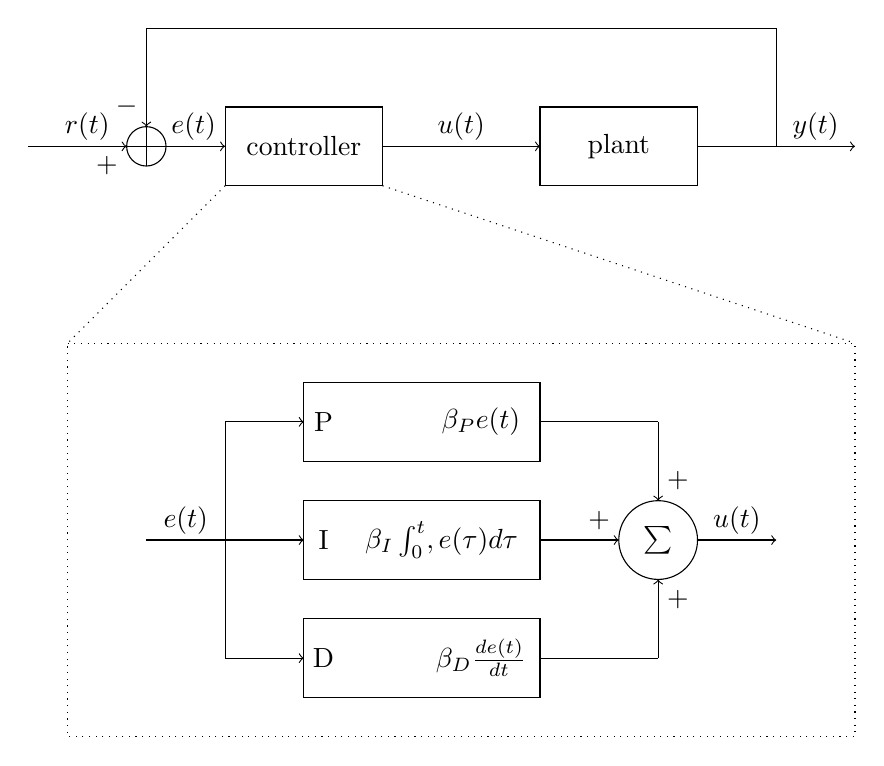
\begin{tikzpicture} 
  \draw (3,1) -- (1,1) -- (1,2) -- (3,2) -- cycle;
  \draw [->] (3,1.5) -- (5,1.5);
  \draw (7,1) -- (5,1) -- (5,2) -- (7,2) -- cycle;
  \draw [->] (7,1.5) -- (9,1.5);
  \draw (8,1.5) -- (8,3) -- (0,3);
  \draw [->] (0,3) -- (0,1.75);
  \draw (0,1.5) circle [radius=0.25];
  \draw (0,1.75) -- (0,1.25);
  \draw (-0.25, 1.5) -- (0.25, 1.5);
  \draw [->] (0.25,1.5) -- (1,1.5);
  \draw [->] (-1.5,1.5) -- (-0.25, 1.5);
  \draw (0.6,1.75) node {$e(t)$};
  \draw (-0.75,1.75) node {$r(t)$};
  \draw (4,1.75) node {$u(t)$};
  \draw (8.5,1.75) node {$y(t)$};
  \draw (2, 1.5) node {controller};
  \draw (6, 1.5) node {plant};
  \draw (-0.25,2) node {$-$};
  \draw (-0.5,1.25) node {$+$};
  
  \draw [dotted] (1, 1) -- (-1, -1);
  \draw [dotted] (3, 1) -- (9, -1);
  \draw [dotted] (-1,-1) -- (9,-1) -- (9,-6) -- (-1,-6) -- cycle;
  \draw (0,-3.5) -- (1,-3.5);
  \draw (1,-5) -- (1,-2);
  \draw [->] (1,-3.5) -- (2,-3.5);
  \draw [->] (1,-2) -- (2,-2);
  \draw [->] (1,-5) -- (2,-5);
  \draw (2, -1.5) -- (5, -1.5) -- (5, -2.5) -- (2, -2.5) -- cycle;
  \draw (2, -3) -- (5, -3) -- (5, -4) -- (2, -4) -- cycle; 
  \draw (2, -4.5) -- (5, -4.5) -- (5, -5.5) -- (2, -5.5) -- cycle;
  \draw (2.25,-3.5) node {I};
  \draw (3.75,-3.5) node {$\beta_I\int_0^t, e(\tau) d\tau$};
  \draw (4.25,-2) node {$\beta_P e(t) $};
  \draw (2.25,-2) node {P};
  \draw (2.25,-5) node {D};
  \draw (4.25,-5) node {$\beta_{D} \frac{de(t)}{dt}$};
  \draw (5, -5) -- (6.5,-5);
  \draw (5, -2) -- (6.5,-2);
  \draw [->] (6.5,-2) -- (6.5, -3);
  \draw [->] (6.5,-5) -- (6.5, -4);
  \draw [->] (5, -3.5) -- (6,-3.5);
  \draw (6.5, -3.5) circle [radius=0.5];
  \draw (6.5, -3.5) node {$\sum$};
  \draw [->] (7,-3.5) -- (8, -3.5);
  \draw (0.5,-3.25) node {$e(t)$};
  \draw (7.5,-3.25) node {$u(t)$};
  \draw (6.75,-2.75) node {$+$};
  \draw (6.75,-4.25) node {$+$};
  \draw (5.75,-3.25) node {$+$};
\end{tikzpicture}


%Plate In A Newtonian Fluid
%%Plate In A Newtonian Fluid
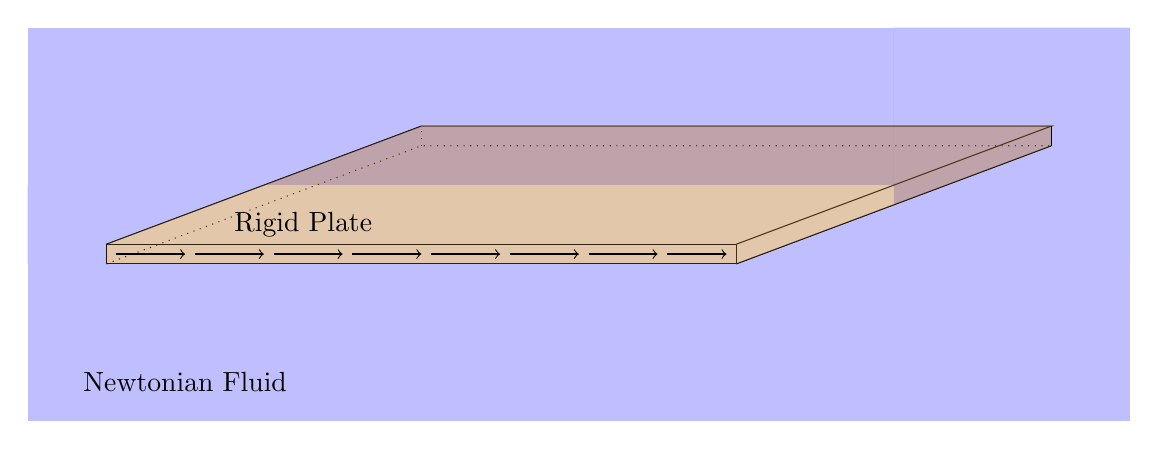
\begin{tikzpicture} 
	\path [fill, color=blue, opacity=0.25] (0,1) -- (14,1) -- (14,-1) -- (0, -1) -- cycle;
	\path [fill, color=blue, opacity=0.25] (9,1) -- (11, 1.75) -- (11, 4) -- (14, 4) -- (14,1) -- cycle;
	\path [fill, color=blue, opacity=0.25] (0,1) -- (1,1) -- (1,1.25) -- (3,2) -- (0,2) -- cycle;
	\path [fill, color=blue, opacity=0.25] (0,2) -- (0,4) -- (11,4) -- (11,2) -- cycle;
	\path [fill, color=brown, opacity=0.25] (1,1) -- (9,1) -- (9,1.25) -- (1, 1.25) -- cycle;	
	\draw (1,1) -- (9,1) -- (9,1.25) -- (1, 1.25) -- cycle;
	\draw [dotted] (1,1) -- (5,2.5) -- (13, 2.5);
	\draw (13,2.5) -- (9,1);
	\draw (1,1.25) -- (5,2.75) -- (13, 2.75) -- (9, 1.25);
	\path [fill, color=brown, opacity=0.25] (1,1.25) -- (5,2.75) -- (13, 2.75) -- (9, 1.25) -- cycle;
	\path [fill, color=brown, opacity=0.25] (1,1) -- (1,1.25) -- (5,2.75) -- (5,2.5) -- cycle;
	\path [fill, color=brown, opacity=0.25] (5,2.5) -- (5,2.75) -- (13,2.75) -- (13,2.5) -- cycle;
	\path [fill, color=brown, opacity=0.25] (9, 1) -- (9,1.25) -- (13,2.75) -- (13,2.5) -- cycle;
	\path [fill, color=brown, opacity=0.25] (1,1) -- (5,2.5) -- (13, 2.5) -- (9, 1) -- cycle;
	\draw (13,2.75) -- (13, 2.5);
	\draw [dotted] (5,2.5) -- (5,2.75);
 	\draw [->] (1.125,1.125) -- (2, 1.125);
 	\draw [->] (2.125, 1.125) -- (3, 1.125);
 	\draw [->] (3.125, 1.125) -- (4, 1.125);
 	\draw [->] (4.125, 1.125) -- (5, 1.125);
 	\draw (2,-0.5) node {Newtonian Fluid};
 	\draw (3.5,1.5) node {Rigid Plate};
 	\draw [->] (5.125, 1.125) -- (6, 1.125);
 	\draw [->] (6.125, 1.125) -- (7, 1.125);
 	\draw [->] (7.125, 1.125) -- (8, 1.125);
 	\draw [->] (8.125, 1.125) -- (8.875, 1.125);
% 	\path [fill, color=blue, opacity=0.5] (0,2) -- (14,2) -- (14,5) -- (0, 5) -- cycle;
\end{tikzpicture}

%PID Controller Explanatory Graph
%PID Controller Explanatory Graph
\begin{tikzpicture} 
  \draw[->] (-1,0) -- (4.2,0) node[right] {$t$};
  \draw[->] (0,-1) -- (0,4.2) node[above] {$e(t)$};
  \draw[scale=0.5,domain=0:8,smooth,variable=\x,blue] plot ({\x},{5*exp(-0.5*\x)*cos(100*\x)});
\end{tikzpicture}


We will consider this in two senses, formally and with a block diagram. The block diagrams are common in engineering for describing these control systems and given their
utility we will make use of them here as well.

Formally we say that we calculate a control value (function) $ u $ by

\begin{align*}
	u(t) = \beta_{P} e(t) + \beta_{D}\frac{de(t)}{dt} + \beta_{I} \int_{0}^{t} e(s) ds
\end{align*}


\bibliographystyle{plain}
\bibliography{references}
\end{document}
